\documentclass[letterpaper, 10 pt, conference]{ieeeconf}
%\documentclass[a4paper, 10pt, conference]{ieeeconf}

\overrideIEEEmargins

\usepackage[utf8]{inputenc}
\usepackage[T1]{fontenc}
\usepackage{hyperref}
\usepackage{graphicx}
\usepackage{ngerman}

\title{\LARGE \bf
FireForceDefense
}

\author{Cameron Barbee, Tim Hoffmann,  Christian Piffel,  Tobias Schotter,\\  Sebastian Schuscha,  Philipp Stangl,  Thomas Stangl%
}

\begin{document}

\maketitle
\thispagestyle{empty}
\pagestyle{empty}

\section{EINLEITUNG}

FireForceDefense ist ein webbasiertes Singleplayer- Tower-Defense Spiel.  Es wurde im Rahmen der Studienarbeit für das Studienfach \textit{Projektmanagement und Agile Entwicklungsmethoden} von Thomas Amman, Cameron Barbee,  Tobias Schotter,  Sebastian Schuscha,  Philipp Stangl und Thomas Stangl initial angefertigt.  Die Projektarbeit im Studienfach \textit{Web Anwendungsentwicklung} soll nun dazu dienen,  das Spielerlebnis zu maximieren.  Aufgrund der zeitlichen Rahmenbedingungen des Projekts im vierten Semester konnten administrative Funktionalitäten wie eine Benutzerverwaltung nicht im vollen Umfang implementiert werden.  \\


Im Gegensatz zu anderen Tower-Defense Spielen gibt es anstelle von Monstern oder anderen beweglichen Gegenständen als Feind ein sich immer weiter ausbreitendes Feuer.  Flammen kommen beispielsweise vom äußeren Rand her oder werden durch (Wald-)Brand, Feuerpfeile, Bomben usw. ausgelöst. Das Feuer lässt sich auf verschiedene Arten,  z. B.  mit einem Löschschiff, bekämpfen bzw.  löschen.  Dabei gilt es die 3 Schutzobjekte (Hauptbasis und zwei weitere Gebäude) vor dem sich ausbreitenden Feuer zu schützen.  Die Ausbreitung des Feuers sowie die Feuerintensität und Brenndauer werden von dem jeweiligen Zelltyp und Zellinhalt beeinflusst. 
Außerdem ist die Kartenstruktur des Spielfelds in hexagonalen Zellen aufgebaut.  Es gibt keine festen Start- und Zielpunkte, von denen Gegner-Wellen kommen können.  Statt Gegner-Wellen gibt es die Effekte (Feuerball,  Blitz und Lava), die an vom Spieler unvorhergesehenen Stellen auftreten können.

Das Spiel basiert auf einem 3-Sterne-Level-System.  Im Verlauf des Spiels durchquert der Spieler eine Insel vom Ufer bis hin zu einem Vulkan, wobei jedes fortgeschrittenere Level einen immer höheren Schwierigkeitsgrad aufweist. Die Hauptbasis,  die zu Beginn eines Levels im Zentrum des Spielfeldes vom Spieler frei platziert werden kann, muss mindestens erhalten bleiben, um einen Stern zu bekommen. Dieser ist zugleich das Kriterium zum Freischalten des nächsten Levels.  Die beiden anderen Sterne können für das Beschützen von zwei weiteren Gebäuden, die nicht frei platzierbar sind, erhalten werden.  Der Bau von Löscheinrichtungen kostet \glqq{}In-Game\grqq{}-Währung, wofür dem Spieler zu Beginn ein Startkapital zur Verfügung steht.  Pro Zeiteinheit und gelöschtem Feuer erhält der Spieler einen festgelegten Betrag als Belohnung gutgeschrieben.  Das Geld ist nicht in andere Level übertragbar.\\


Ziel bei der Entwicklung und bei der späteren Verwendung ist die Plattformunabhängigkeit.  Daraus ergeben sich folgende technische Schlüsselbausteine:
\begin{itemize}
\item Frontend-Framework: Vue.js
\item Modul-Packer und Dev-Server: Webpack
\item API: REST
\item Backend: NodeJS mit TypeScript und Express
\item Containerisierung: Docker
\end{itemize}

\section{VERWANDTE ARBEITEN}
Die hexagonale Kartenstruktur ist inspiriert durch das Spiel „Battle For Wesnoth“.

\begin{figure}[thpb]
      \centering
      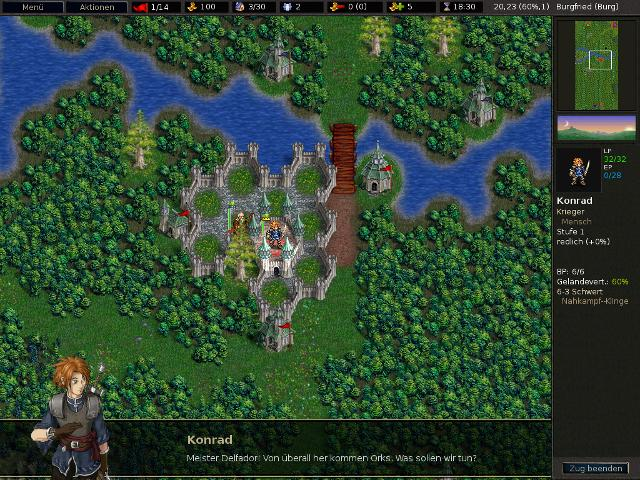
\includegraphics[scale=0.38]{images/spielszene}
      \caption{Beispiel für hexagonale Kartenstruktur (Quelle: \href{https://media-cdn.ubuntu-de.org/wiki/attachments/44/11/Spielszene.jpg}{media-cdn.ubuntu-de.org/wiki/attachments/44/11/Spielszene.jpg})}
      \label{figurelabel}
\end{figure}

\section{ANFORDERUNGEN}

Es gibt drei primäre Ziele, die es während der Projektarbeit umzusetzen gilt: (1) Die Zusammenführung der Codebase zu einer Monorepo, (2) die Cloudfähigkeit der Anwendung,  und (3) die Möglichkeit zur Registrierung,  Anmeldung,  Speicherung des Spielstands und Anzeige der Rangliste für ein gesteigertes Spielerlebnis.  

Ein optionales Ziel ist die Integration einer Benutzerverwaltung.

\subsection{Monorepo}

Als Entwickler möchte ich ein Monorepo, damit ich zu jeder Zeit einen konsistenten Stand des Gesamtprojekts habe.  Akzeptanzkriterien sind:
\begin{itemize}
\item Der Code von Backend und Frontend liegt vollständig im Repository vor.
\item Durch eine Kennzeichnung ist ersichtlich zu welchem Zeitpunkt der neue Code von dieser Projektarbeit hinzukommt. 
\item Building-,Test- und Linting-Tools sind konfiguiert und funktionieren.
\item Das Backend und Frontend funktionieren wie vor der Zusammenführung in ein Monorepo.
\item Eine Gitlab-Pipeline zum Ausführen der Linting- und Testing-Tools ist eingerichtet.
\item Im Repository ist eine Anleitung zur lokalen Projekteinrichtung hinterlegt.
\end{itemize}

\subsection{Cloud-Kompatibilität}

Als DevOps-Engineer möchte ich eine Cloud-kompatible Anwendung für eine problemlose Bereitstellung der Anwendung.  Akzeptanzkriterien sind:
\begin{itemize}
\item Ein Dockerfile ist erstellt und lauffähig.
\item Alle notwendigen Anpassungen zur Erstellung und Deployment des Docker-Images sind der GitLab-Pipeline vorgenommen.
\item Das Backend ist per Umgebungsvariable konfiguierbar.
\item Eine grundlegende Secrets-Verwaltung zur sicheren Aufbewahrung von Zugangsinformationen ist eingerichtet.
\item Die prinzipielle Erreichbarkeit ist sichergestellt,  sodass bei der Abschlusspräsentation eine Demo des Spiels in der Cloud möglich ist.
\item Die eingeschränkte Erreichbarkeit des Spiels in der Cloud ist dokumentiert.
\end{itemize}

\subsection{Spielstand-Speicherung}

Als Spieler möchte ich meinen Spielstand speichern können,  damit ich zu einem späteren Zeitpunkt im Spielverlauf fortfahren kann,  anstatt neu starten zu müssen.  Akzeptanzkriterien sind:
\begin{itemize}
\item Der Spielstand wird über die RESTful-API gespeichert.
\item Eine Datenbank(-tabelle) für die Spielstände ist angelegt.
\item Gespeichert wird:
\begin{itemize}
\item Zeitpunkt
\item Benutzer
\item Level
\item Sterne
\item Geld
\item Dauer
\item Abgebrannte Fläche
\end{itemize}
\item Es soll keine Benutzerinteraktion nötig sein.  Die Speicherung des Spielstand erfolgt am Ende des Levels automatisch.
\item (Optional) Eine Plausibilitätsprüfung der zu speichernden Daten.
\end{itemize}

\subsection{Registrierung}

Als Spieler möchte ich mich registrieren können,  damit Account-spezifische Daten mit meinem Account in Verbindung gebracht werden können.  Akzeptanzkriterien sind:
\begin{itemize}
\item Die Registrierung erfolgt mit E-Mail-Adresse,  Benutzername und Passwort.
\item Sowohl E-Mail als auch Benutzername sind jeweils eindeutig im System identifizierbar.
\item Die Wireframes vom Prototyping der Benutzerführung bei der Registrierung sind vorhanden.
\item Im Frontend ist eine Ansicht zur Registrierung implementiert.
\item Ein \glqq{}Passwort wiederholen\grqq{}-Feld ist eingebaut.
\item Eine Datenbank(-tabelle) für den Benutzer ist erstellt.
\item Die Registrierung wird über die RESTful-API gespeichert.
\item E-Mail und Benutzername werden mit RegEx validiert. 
\item (Optional) Die angegebene E-Mail wird verifiziert.
\end{itemize}

\subsection{Anmeldung}

Als Spieler möchte ich mich anmelden können,  um auf meine Account-spezifischen Daten zugreifen zu können.  Akzeptanzkriterien sind:
\begin{itemize}
\item Die Anmeldung erfolgt mit E-Mail-Adresse,  oder Benutzername, und Passwort.
\item Die Wireframes vom Prototyping der Benutzerführung bei der Anmeldung sind vorhanden.
\item Die Anmeldung erfolgt über die RESTful-API.
\item Für Frontend und Backend gibt es eine Sitzungsverwaltung.
\item Im Frontend ist eine Ansicht zur Anmeldung implementiert.
\item Die Abmeldung erfolgt über die Sitzungsverwaltung.
\item (Optional) Sollte man das Passwort vergessen haben, kann man einen Link zum Zurücksetzen des Passworts an die im Account hinterlegte E-Mail-Adresse anfordern.
\item (Optional) Es gibt eine Option um angemeldet zu bleiben.  Der Sitzungstoken wird als Cookie im Internet-Browser hinterlegt.
\end{itemize}

\subsection{Rangliste}

Als Spieler möchte ich eine Rangliste,  damit ich mich mit anderen Spielern vergleichen kann.  Akzeptanzkriterien sind:
\begin{itemize}
\item Die Wireframes des Prototypings sind vorhanden.
\item Die Rangliste ist im Frontend implementiert.
\item Die Sortierung erfolgt anhand der Kriterien:
\begin{itemize}
\item Sterne
\item Dauer
\item Verfügbares Geld
\item Abgebrannte Fläche
\end{itemize}
\item Es kann entweder eine Gesamt-Rangliste oder eine nach Level gefilterte Rangliste angezeigt werden.
\item Sortierkriterien und Filter sind im Backend der Anwendung implementiert.
\item Der eigene Ranglisteneintrag wird fixiert angezeigt.
\item Die Abfrage der Daten erfolgt über die RESTful-API.
\item (Optional) Es kann nach Spielern in der Rangliste gesucht werden.
\end{itemize}

\subsection{(Optional) Benutzerverwaltung}

Als Benutzer möchte ich eine Benutzerverwaltung,  damit ich Änderungen an meinem Benutzeraccount vornehmen kann. 

\subsection{Testabdeckung}

Als Entwickler möchte ich eine ausreichende Testabdeckung,  damit Fehler frühzeitig erkannt werden.  Akzeptanzkriterien sind:
\begin{itemize}
\item Alter,  bisher nicht von Tests abgedeckter Code bekommt Tests.
\item Die Abdeckungsrate liegt bei mindestens 50\%.
\item Vue-Components werden durch ein geeignetes Werkzeug getestet, beispielsweise mit \textit{vue-test-utils}.
\end{itemize}

\section{METHODEN}
Für die Repräsentation des Spiels im client-seitigen Frontend wird das Framework Vue.js verwendet.  Zur Speicherung der Daten kommt voraussichtlich SQLite zum Einsatz. Zwischen den beiden Instanzen befindet sich ExpressJS, mit Node.js als Laufzeitumgebung, im server-seitigen Backend.  Die Kommunikation zwischen Frontend und Backend wird über eine RESTful-API abgewickelt.
Die Bibliothek Lottie sorgt für eine grapfisch anspruchsvolle Repräsentation der Animationen. 
Um eine fehlerfreie Anwendung zu entwickeln wird zum einen TypeScript als projektweite Programmiersprache verwendet.  Dadurch sollen Fehler bereits zur Kompilierzeit identifiziert werden können.  Zum Anderen wird das Test-Framework Jest für Unit-Tests verwendet. 
Das Spiel wird in einem Docker Container bei einem Cloud-Anbieter (Amazon Web Services) bereitgestellt.

\addtolength{\textheight}{-12cm} 

\end{document}